\documentclass[a4paper]{article}
\usepackage{fontspec}
\usepackage{amsmath}
\usepackage{amssymb}


%%%%lualatex on
%\usepackage{luatextra}
%Ligatures={Contextual, Common, Historical, Rare, Discretionary}
%\setmainfont[Mapping=tex-text]{Linux Libertine O}

\usepackage{natbib}

\title{Note about WSC}
\author{Simon}
\begin{document}
\maketitle
\section{Cultural Evolution}


We run a first set of experiment where all agents interact with everyone. The only evolutionary mechanism are. Following \cite{bentley2004randomdriftandculturechange}

The cultural evolution's literature gives us a way to interpret evolution of cultural artifact such as those produce in economical field. We want to confront well know cultural evolution's mechanism to well known economical evolution's mechanism and see and show their differences.

To do so we cross those different mechanisms following the table \ref{tab:exp}.
\begin{table}
	\centering
	\begin{tabular}{l|c|c}
		& Eco\footnote{a} & Rand \\\hline
		$\mu$ &A & B \\
		$\alpha$ & B & C \\
	\end{tabular}
	\caption{Experimental Setup}
	\label{tab:exp}
\end{table}

\subsection{One trait}

The Finite Innovation Effect (ie : $n$ variant  $| n\in\{0,\cdots,100\}$). If choose a innovation mechanism such as the number of possible new variant is finite, we see a strange ``anticonformist-like'' effect such the one shown by \cite{mesoudi2009randomcopyingfrequencydependencopyingandulturechange}. This effect is visible in the figure \ref{fig:finitEffect}.
\begin{figure}[h]
	\begin{center}
		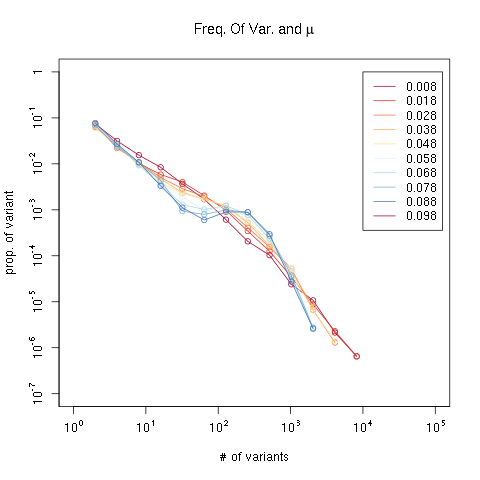
\includegraphics[width=7cm]{img/allmu.png}
	\end{center}
	\caption{rand()\%100}
	\label{fig:finitEffect}
\end{figure}


With infinite innovation possibilities(ie : $n$ variant $| n\in\mathbb{A} $) the results, showed in the figure \ref{fig:allMutation} are the same that those from \cite{bentley2004randomdriftandculturechange}.
\begin{figure}[hbp]
	\begin{center}
		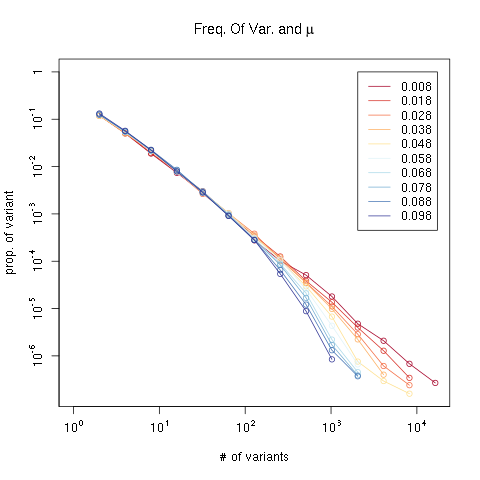
\includegraphics[width=7cm]{img/allmuRandMax.png}
	\end{center}
	\caption{rand()\%RAND\_MAX}
	\label{fig:allMutation}
\end{figure}


\section{Multiple Traits (all varying on $\mathbb{N}$)}
In that case individual owns a vector of $n$ traits. One a cultural exchange occurs the whole vector is exchanged.

In the case individual carries multiples traits (ie price in our experiment), we check that it does not change the result of the algorithm in the long terms, each traits will evolve following the same curves than when just one trait is evolving. The results are shown in figures \ref{fig:10resources}. Those results are statistically the same than those from the previous experiments.
\begin{figure}[h]
	\begin{center}
		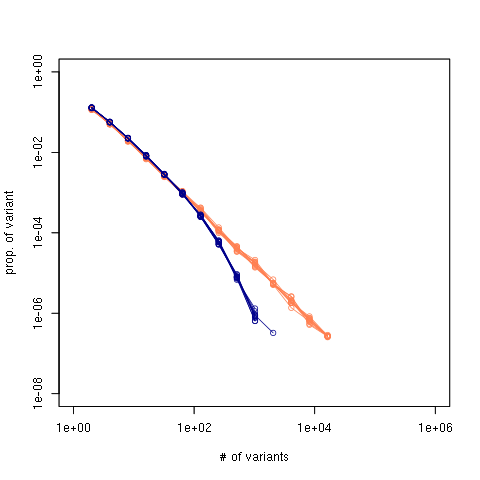
\includegraphics[width=6cm]{img/10resources.png}
	\end{center}
	\caption{$\mu=\{.08,.098\}$ for 10 resources}
	\label{fig:10resources}
\end{figure}

\begin{figure}[h]
	\begin{center}
		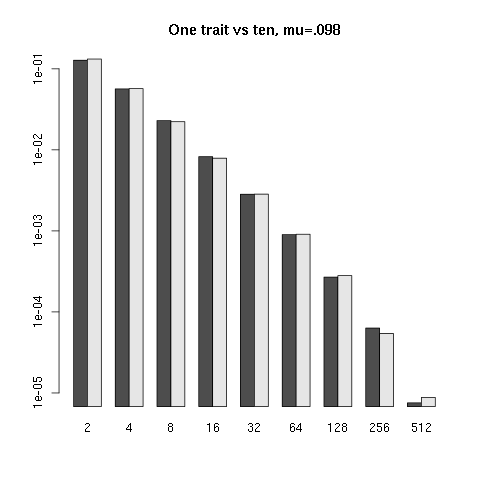
\includegraphics[width=6cm]{img/OneVsTenMu098.png}
		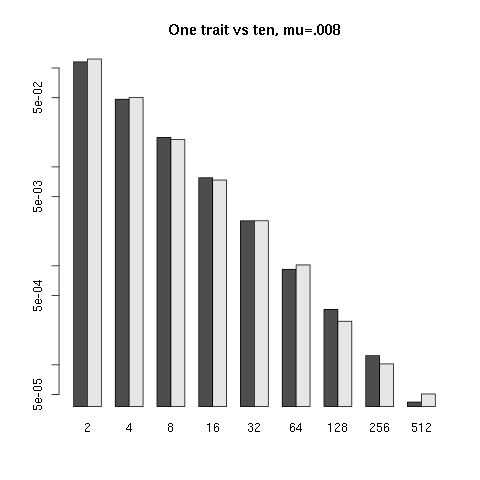
\includegraphics[width=6cm]{img/OneVsTenMu008.png}
	\end{center}
	\caption{$\mu=\{.08,.098\}$ for one of the 10 resources VS one only}
	\label{fig:OneVsTen}
\end{figure}

\bibliographystyle{apalike}
\bibliography{/home/scarrign/Documents/biblio/bib/phd.bib}  
\end{document}


